% Part 2: Easy Problems with Hints (2 problems)

% Problem 1: Complex Locus (Sample 19)
\begin{problem}[Distance Ratio Regions]
Let $z_1 = 2 + i$ and $z_2 = -1 + 2i$. Sketch the region in the complex plane where:
\[ \frac{|z - z_1|}{|z - z_2|} < 1 \]
\end{problem}

\begin{hint}
Consider the geometric interpretation of $|z - z_1|/|z - z_2| < 1$. This represents the locus where one distance is smaller than another.
\end{hint}

\begin{solution}
The inequality $\frac{|z - z_1|}{|z - z_2|} < 1$ is equivalent to $|z - z_1| < |z - z_2|$.
This means point $z$ is closer to $z_1 = 2 + i$ than to $z_2 = -1 + 2i$.
The locus of points equidistant from two points is the perpendicular bisector of the line segment joining them.
The midpoint of $z_1z_2$ is $\frac{(2+i) + (-1+2i)}{2} = \frac{1 + 3i}{2}$.
The direction vector is $z_2 - z_1 = (-1+2i) - (2+i) = -3 + i$.
The perpendicular bisector has normal vector $-3 + i$.
The region where $|z - z_1| < |z - z_2|$ is the half-plane containing $z_1$.
\begin{center}
    \begin{tikzpicture}[scale=0.9]
        % Axes
        \draw[->] (-3.5,0) -- (4.5,0) node[below right]{$x$};
        \draw[->] (0,-2.5) -- (0,3.5) node[above left]{$y$};

        % Points z1 and z2
        \coordinate (zone) at (2,1);
        \coordinate (ztwo) at (-1,2);
        \fill[fill=blue!70] (zone) circle (2.2pt) node[below right]{$z_1=(2,1)$};
        \fill[fill=red!70] (ztwo) circle (2.2pt) node[above left]{$z_2=(-1,2)$};

        % Segment z1-z2
        \draw[thick] (zone) -- (ztwo);

        % Midpoint and perpendicular bisector
        \coordinate (mid) at ($(zone)!0.5!(ztwo)$);
        \fill (mid) circle (1.5pt) node[below right]{$M=\left(\tfrac{1}{2},\tfrac{3}{2}\right)$};
        % Direction vector from z2-z1 = (-3,1); perpendicular direction (1,3)
        \draw[very thick,color=teal!80!black] ($(mid)+(-2, -6)$) -- ($(mid)+(2, 6)$) node[above right]{bisector};

        % Half-plane closer to z1 (shade lightly)
        \path[fill=blue!10] (zone) -- (ztwo) -- ($(mid)+(2,6)$) -- ($(mid)+(-2,-6)$) -- cycle;
        \node at (2.8,2.8) {\small $|z-z_1|<|z-z_2|$};
    \end{tikzpicture}
\end{center}
\end{solution}

\begin{takeaways}
\begin{enumerate}
    \item \textbf{Distance Comparison:} The locus $|z-a| = |z-b|$ is the perpendicular bisector of segment $ab$.
    \item \textbf{Half-Plane Regions:} Inequality $|z-a| < |z-b|$ defines the half-plane containing $a$.
\end{enumerate}
\end{takeaways}

% Problem 2: Orthocenter via Vectors (Sample 02 - New)
\begin{problem}[Orthocenter Vector Identity]
Let $ABC$ be a triangle with circumcentre $O$, and set
\[\vec{OA}=\mathbf{a},\qquad \vec{OB}=\mathbf{b},\qquad \vec{OC}=\mathbf{c}.
\]
Define the point $H$ by
\[\vec{OH}=\mathbf{a}+\mathbf{b}+\mathbf{c}.
\]
Show that $\vec{BH}\perp\vec{AC}$.
\end{problem}

\begin{hint}
Express $\vec{BH}$ and $\vec{AC}$ in terms of $\mathbf{a},\mathbf{b},\mathbf{c}$ and compute their dot product. Use that $|\mathbf{a}|=|\mathbf{c}|$ since $O$ is the circumcentre.
\end{hint}

\begin{solution}
Compute
\[\vec{BH}=\vec{OH}-\vec{OB}=(\mathbf{a}+\mathbf{b}+\mathbf{c})-\mathbf{b}=\mathbf{a}+\mathbf{c},\]
and
\[\vec{AC}=\vec{OC}-\vec{OA}=\mathbf{c}-\mathbf{a}.
\]
Their dot product is
\[(\mathbf{a}+\mathbf{c})\cdot(\mathbf{c}-\mathbf{a})=|\mathbf{c}|^2-|\mathbf{a}|^2=0,
\]
since $|\mathbf{a}|=|\mathbf{c}|$ (both equal the circumradius). Hence $\vec{BH}\perp\vec{AC}$.

\begin{center}
    \begin{tikzpicture}[scale=1.2]
        % Circumradius
        \def\R{2}
        % Points
        \coordinate (O) at (0,0);
        \coordinate (A) at ({110}:\R);
        \coordinate (B) at ({200}:\R);
        \coordinate (C) at ({340}:\R);
        % H = A+B+C (vector sum)
        \coordinate (H) at ($(A)+(B)+(C)$);
        % Draw circle and triangle
        \draw[gray,thin] (O) circle (\R);
        \draw[thick] (A) -- (B) -- (C) -- cycle;
        % Vectors OA,OB,OC and OH
        \draw[->,blue,thick] (O) -- (A) node[midway,left]{$\mathbf{a}$};
        \draw[->,blue,thick] (O) -- (B) node[midway,below]{$\mathbf{b}$};
        \draw[->,blue,thick] (O) -- (C) node[midway,right]{$\mathbf{c}$};
        \draw[->,red,very thick] (O) -- (H) node[midway,right]{$\vec{OH}$};
        % BH dashed and foot projection to AC
        \draw[dashed,red] (B) -- (H) node[midway,above right]{$\vec{BH}$};
        \draw[dashed,gray] (B) -- ($(A)!(B)!(C)$);
        % Labels
        \node[above] at (A) {$A$};
        \node[below left] at (B) {$B$};
        \node[below right] at (C) {$C$};
        \node[below] at (O) {$O$};
        \node[above right] at (H) {$H$};
    \end{tikzpicture}
\end{center}

\end{solution}

\begin{takeaways}
\begin{enumerate}
    \item \textbf{Vector orthocenter:} The identity $\vec{OH}=\vec{OA}+\vec{OB}+\vec{OC}$ characterises the triangle's orthocentre relative to the circumcentre.
    \item \textbf{Dot-product trick:} Use $(\mathbf{u}+\mathbf{v})\cdot(\mathbf{v}-\mathbf{u})=|\mathbf{v}|^2-|\mathbf{u}|^2$ when equal magnitudes appear.
\end{enumerate}
\end{takeaways}

% Problem 3: Complex Regions (Sample 20)
\begin{problem}[Imaginary Part Constraints]
Sketch the region in the complex plane where:
\[ \text{Im}(2z + 3\bar{z}) \ge 1 \]
\end{problem}

\begin{hint}
For a linear combination $az + b\bar{z}$, the imaginary part has a specific geometric interpretation in the complex plane.
\end{hint}

\begin{solution}
Let $z = x + iy$, so $\bar{z} = x - iy$.
\begin{align*}
2z + 3\bar{z} &= 2(x + iy) + 3(x - iy) \\
&= 2x + 2iy + 3x - 3iy \\
&= 5x - iy
\end{align*}
Therefore, $\text{Im}(2z + 3\bar{z}) = -y$.
The constraint becomes $-y \ge 1$, which is equivalent to $y \le -1$.
This is the region below the horizontal line $y = -1$.
\begin{center}
    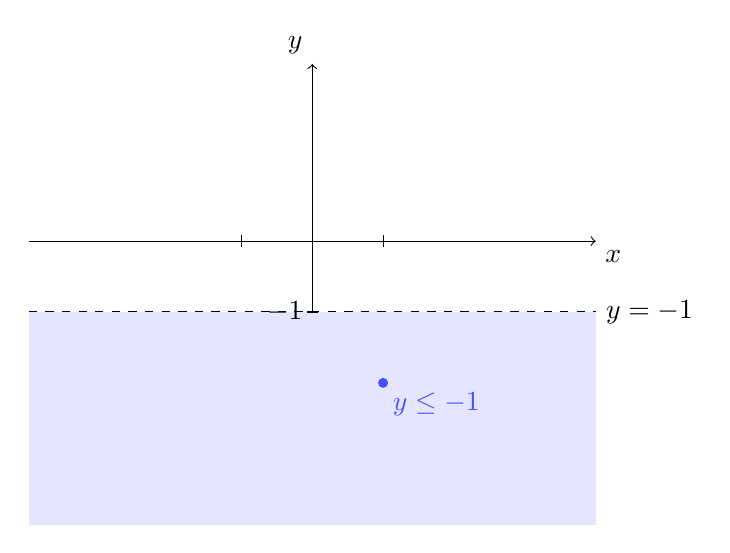
\begin{tikzpicture}[scale=0.9]
        % Axes
        \draw[->] (-4,0) -- (4,0) node[below right]{$x$};
        \draw[->] (0,-4) -- (0,2.5) node[above left]{$y$};

        % Boundary line y = -1 (dashed)
        \draw[dashed, thick] (-4,-1) -- (4,-1) node[right]{$y=-1$};

        % Shade half-plane y \le -1
        \path[fill=blue!10] (-4,-4) -- (4,-4) -- (4,-1) -- (-4,-1) -- cycle;

        % Example point in region
        \fill[blue!70] (1,-2) circle (2pt) node[below right]{$y\le -1$};

        % Tick marks for clarity
        \draw (0,-1) node[left]{$-1$} ++(-0.08,0) -- ++(0.16,0);
        \draw (1,0) ++(0,-0.08) -- ++(0,0.16);
        \draw (-1,0) ++(0,-0.08) -- ++(0,0.16);
    \end{tikzpicture}
\end{center}
\end{solution}

\begin{takeaways}
\begin{enumerate}
    \item \textbf{Linear Combinations:} For $az + b\bar{z}$ with $z = x + iy$, substitute and collect real/imaginary parts.
    \item \textbf{Half-Plane Regions:} Constraints on $\text{Im}(...)$ or $\text{Re}(...)$ typically define half-planes.
\end{enumerate}
\end{takeaways}